%!TEX root = thesis.tex

\chapter{A population of ``clumpy'' galaxies in local Universe}\label{chap:5}
Simultaneous to the development of this research was the publishing of the Galaxy Zoo: Hubble galaxy morphology classification catalog. A portion of the original GZ2 SDSS galaxy sample was included in Galaxy Zoo: Hubble because the decision tree for the latter was more complex than that for GZ2. This enabled a comparison between different decision trees and led to the identification of a rare sample of low redshift clumpy galaxies. This chapter details the identification of such a sample, preliminary analysis of the star-forming clumps, and methods to identify more such galaxies in the local universe as these may be analogs of high redshift galaxies with similar properties.


\section{Introduction}
Structural properties of typical galaxies today wereforgedover the5billionyearsbetween the peakof the cosmic star-formation history at z ⇠ 1.5  2 and now.From the theoretical perspective,galaxies’ growth is predominantly governed by the baryonic physics of gas accre-tion and energy feedback, rather than by merg-ers that induce starbursts (e.g., Somerville and Dav ́ e, 2015). Gas inflow modulates galaxies’ star formation history and plays a crucial role in the dynamical state of the galaxy.A varying gas fraction changes the amount of fragmentation within the gaseous disk, the star-formation rates (SFR), strengths and lifetimes of disk structural components, and possibly the fueling rate of the AGN. As a consequence of the gas accretion pro-cess, the small-scale structure within disk galax-ies is also predicted to change over time, with the appearance of stable “grand design” spiral arms only at later epochs (e.g. Oppenheimer et al., 2010; Bouch ́ e et al., 2010; Dav ́ e et al., 2011a,b; Lilly et al., 2013; Hirschmann et al., 2013). 

n the theoretical paradigm discussed above, the origin of these massive clumps is still an open debate. Two main physical scenarios have been proposed.On one side (hereafter referred to as in-situ models),giant clumps are expectedto form inside pre-existing galaxies.In these sce-narios, haloes located at the center of multiple filaments continuously accrete gas from the cos-mic web.This accretion results in the forma-tion of gas-dominated disks that eventually frag-ment into giant clumps by gravitational insta-bility (Bournaud et al., 2007; Dekel et al., 2009; Behrendt et al., 2015). On the other side (here-after referred to as ex-situ models) clumps may have an external origin, as in the case of mergers with small star-forming companions (Ceverino et al., 2010; Bournaud, 2016). 

Observationally, the situation is still unclear. The large gas-to-baryonic fraction of 20 to 80 recently measured with interferometric studies in clumpy galaxies lends support to the in-situ models(e.g., Erb et al., 2006; Tacconi et al., 2008, 2010).Similarly, the kinematics in the majorityofthesegalaxiesischaracterized by large, regularly-rotating disks, with no signs of on-going or recent mergers (Genzel et al., 2006; F ̈ orster Schreiber et al., 2009; Epinat et al., 2012; Newman et al., 2012).These studies, however, are 1) limited to galaxies with SFR> 10M yr 1 and M>10 10 M) and 2) include only a few galaxies with high spatial resolution kinematic and interferometric data (Genzel et al., 2014). 

The lack of existing observational constraints below 10 10 M is of particular concern. It is pre-cisely in this mass range that most of the con-straining power resides. In fact, state of the art simulations that directly resolve the interstellar medium of individual galaxies while capturing their cosmological environment show that low mass galaxies are the mostly a↵ected by preven-tive feedback (e.g., FIRE Muratov et al.2015; 11
GASOLINE Christensen et al. 2015; and MU-FASA Dav ́ e et al.2016).These simulations show that in galaxies with M<10 10 supernova-driven fast outflows can lower the gas inflow rate, and consequently the rate at which clumps are formed in-situ, compared to more massive galax-ies. If clumps are the result of minor merging, on the other hand, the dependency with stellar mass would depend on the specifics of the dy-namics of the mergers. 

Throughout this chapter we assume a flat Planck cosmology with H$_0=67.8$ and $\Omega_m = 0.308$ where appropriate. 


\section{Sample Selection \& Data} \label{sec:chap5-sample}

We identify a sample of clumpy galaxies in the local universe by considering classifications from both the Galaxy Zoo 2 \citep[GZ2][]{Willett2013} and Galaxy Zoo: Hubble \citep[GZH][]{Willett2017} projects. We provide a brief overview of each of these projects here. 

The GZ2 subject sample consists of 285,962 galaxies identified as the brightest 25\% ($r$-band magnitude $< 17$) residing in the SDSS North Galactic Cap region from Data Release 7 and included subjects with both spectroscopic and photometric redshifts out to $z < 0.25$. In addition to the DR7 Legacy catalog, galaxies were included from Stripe 82, a multiply-imaged strip along the celestial equator in the Southern Galactic Cap. Galaxies in this region were selected to have $m_r\le17.7$ and petror90\_r $>3$, where petror90\_r is the radius containing 90\% of the r-band Petrosian aperture flux.


\begin{figure}
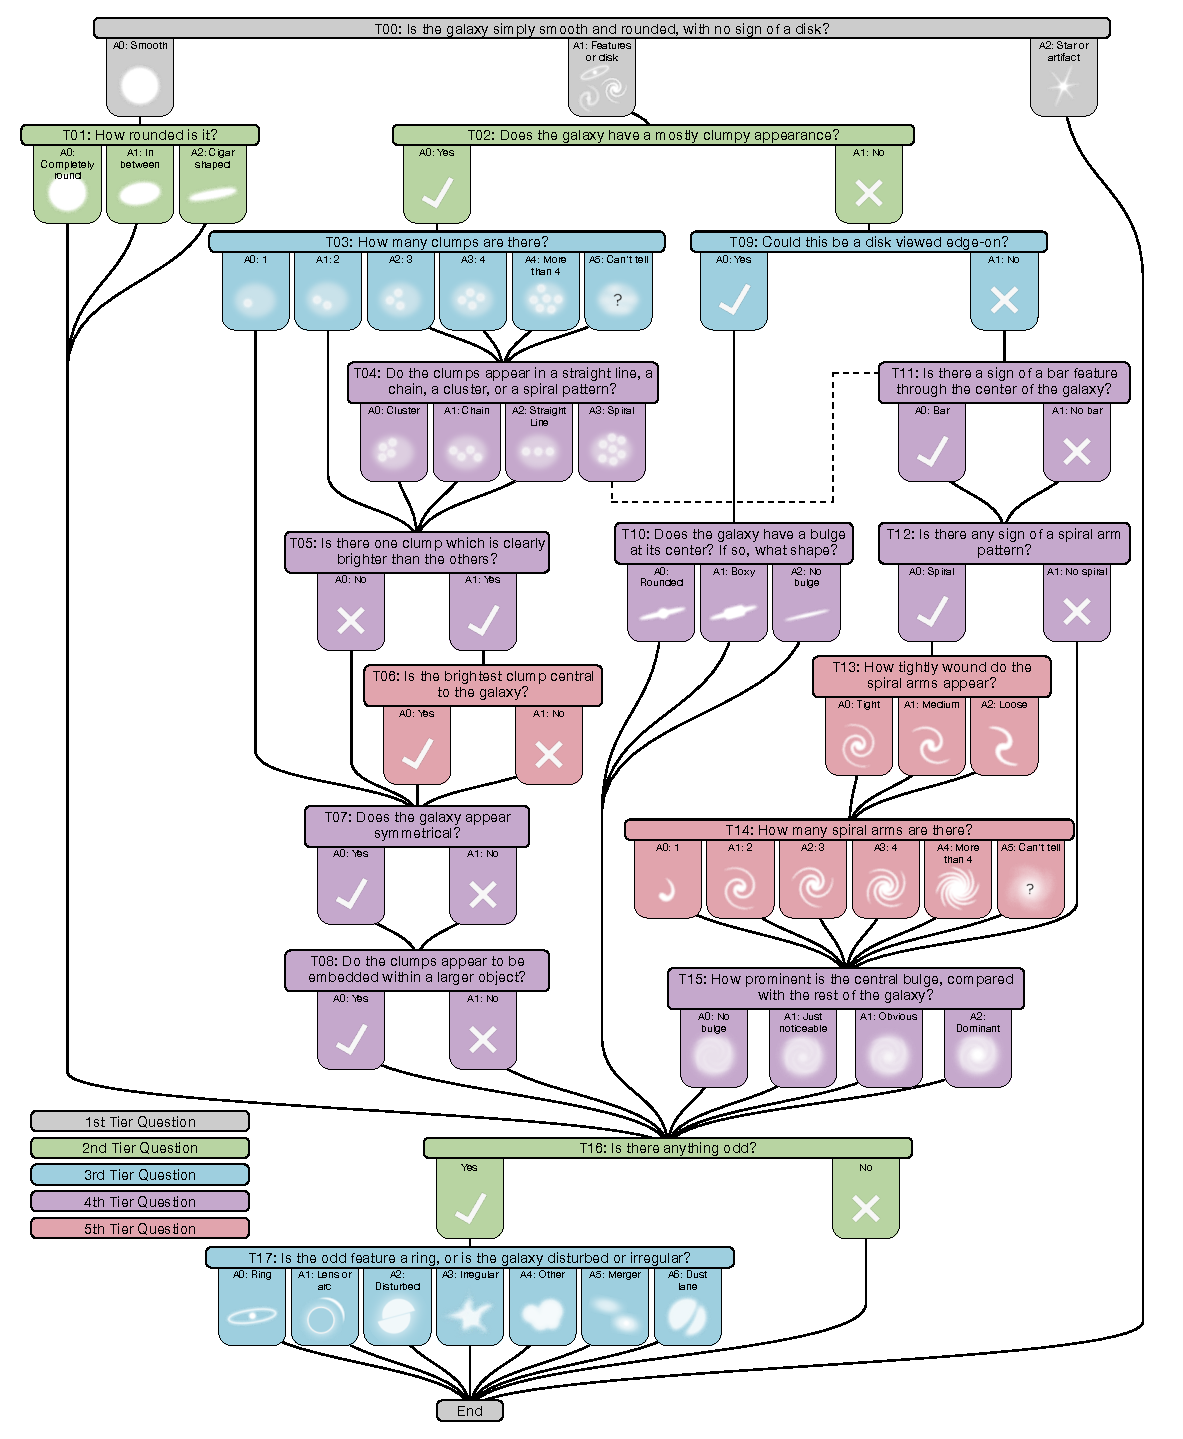
\includegraphics[width=\textwidth]{Figures/gz3_tree_resized.pdf}
\caption[Galaxy Zoo: Hubble decision tree.]{Galaxy Zoo: Hubble decision tree. The most notable difference between this decision tree and that used during the Galaxy Zoo 2 project is the ``clumpy'' branch of tasks.}
\label{fig: gzh decision tree}
\end{figure}

The GZH project contains images drawn from several dedicated surveys and sample selection criteria. Most samples are drawn from various Hubble fields such as AEGIS, GOODS and COSMOS; however also included are the single-epoch and co-added images from Stripe 82 of the SDSS Data Release 7 that were part of the GZ2 project. The single-epoch imaging allows for local comparison to higher redshift galaxies, while the co-added imaging allows for image depth analyses. 

The most notable difference between these two projects is the decision tree presented to volunteers. The goal of GZH was to collect detailed morphologies for galaxies in Hubble imaging which extends to much higher redshift than those of the SDSS sample. Galaxies at higher redshift do not necessarily follow the traditional Hubble sequence and thus a new branch of questioning was added to the decision tree for this project, shown in Figure \ref{fig: gzh decision tree}. This included several questions concerning the clumpy nature of galaxies, a morphological feature well known to exist at higher redshift. Because GZH included galaxies from the GZ2 project, we can draw on both sets of decision trees to identify clumpy features for galaxies in Stripe 82.


To select a sample of ``clumpy" galaxies from the GZH Stripe 82 sample, we consider only those subjects with large featured (\ffeat) and clumpy (\fclump) vote fractions: the fraction of volunteers who voted a subject as `featured or disk' in response to the first question ``Is the galaxy simply smooth and rounded, with no sign of a disk?'' and who answered `yes' to the question ``Does the galaxy have a mostly clumpy appearance?'' Specifically, we select galaxies which satisfy \ffeat~$\ge0.5$ and \fclump~$\ge0.5$ Additionally, we require $N_{\mathrm{votes}} \ge 20$, where $N_{\mathrm{votes}}$ is the number of volunteers who answerd the clumpy question. This insures that \fclump~is statistically significant and not a product of too few votes.  This yields a sample of 629 galaxies: 273 single-epoch imaging and 356 from the co-added imaging. After visual inspection we find that this is hardly a pure sample of clumpy galaxies in the traditional sense, instead including a sizeable sample of tight groups of elliptical galaxies, as well as galaxies in various merging states, possessing multiple nuclei. [\textbf{show example image?}] After excluding these and duplicate imaging, we retain 92 coadd-depth and 105 single-depth clumpy galaxies, of which 156 are unique systems (some objects are common to both the single-epoch and coadd-depth imaging). Finally, we exclude galaxies with $z>0.06$ in order to retain a sample wherein the physical scale as observed by SDSS is similar to Hubble's at $z\sim3$ to allow for comparison with high redshift samples. Our final sample contains 105 unique galaxies. 

\begin{figure}
\centering
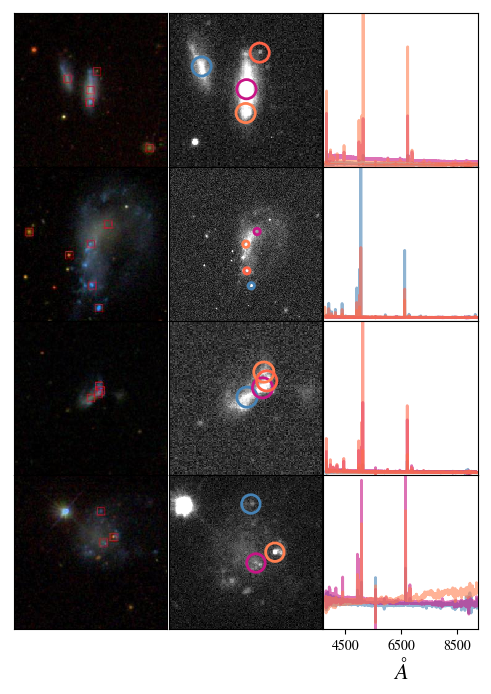
\includegraphics[width=4.75in]{Figures/jpeg_fits_spec_examples.png}
\caption[Sample of ``clumpy'' galaxies determined by Galaxy Zoo: Hubble]{Sample of ``clumpy'' galaxies. The first column shows the SDSS $gri$ color composite image where the red squares denote locations of SDSS spectroscopy. The middle column shows our postage stamp for the object where the colored circles show the same spectral locations, however these circles are color coded to the third panel which shows the spectra associated with each object.}
\label{fig: clumpy examples}
\end{figure}

We obtain SDSS Data Release 12 (DR12) \textit{ugriz} coadd imaging, as well as all optical spectra associated with each galaxy. The wavelength range of the SDSS spectra is $3800-9200$\AA~with a resolution of $R\sim 1500$ at $\sim3800$\AA. The $3$\arcsec~SDSS fibers cover 2.9 kpc at $z=0.05$. We visually inspect all spectra to verify that they are associated with an object in our sample as opposed to a nearby object or overlapping star. Through this inspection we determine that one clumpy galaxy is actually a juxtoposition of three galaxies at disparate redshifts flagged as clumpy in GZH due to the low resolution of SDSS imaging. We exclude this subject from our sample. Our final list includes 171 spectra. Approximately half of the galaxies in our sample have more than one spectrum with a handful having three or four spectra. Figure \ref{fig: clumpy examples} shows some examples of our clumpy galaxies where the first column is the $gri$ color composite SDSS jpeg image with red squares denoting the location of SDSS spectra, the middle column is the $r$-band postage stamp (described below) where the colored circles again denote the location of SDSS spectra and reflect the size of the fiber. The third column shows the spectra associated with each object, color-coded to the apertures in the middle column. 


We create postage stamps of each galaxy from the $r$-band SDSS fields.  The size of the postage stamp is taken to be 3$\times\mathtt{petrorad\_r}$, the Petrosian radius as measured in the $r$-band by the SDSS pipeline. We then run Source Extractor \citep{sextractor} on each postage stamp. During visual inspection of these cutouts and the associated SExtractor segmentation maps we discover that the SDSS coordinates are occasionally incorrectly assigned, that is, star-forming clumps are mistaken for individual galaxies likely due to the low surface brightness of some of these systems. An example is shown in the final row of Figure \ref{fig: clumpy examples}. It is clear in the first panel that the central coordinates are not well aligned with the galactic center. The middle panel depicts our postage stamp in which we have corrected the galaxy's coordinates using that determined by SExtractor. 


We also draw on the \textit{GALEX}-SDSS-\textit{WISE} Legacy Catalog \citep[GSWLC,][]{Salim2016} which provides stellar mass, star formation rates (SFR) and dust attenuations for 700,000 low-redshift galaxies. Specifically we obtain the GSWLC-X version which contains measurements using the deepest imaging available for each galaxy in the sample. We provide a brief overview of their methodology here.  Galaxy physical properties were obtained from UV and optical spectral energy distribution (SED) fitting utilizing imaging data from the \textit{Galaxy Evolution Explorer}, SDSS, and \textit{Wide-field Infrared Survey Explorer} surveys for galaxies with $z<0.3$, covering up to 90\% of the SDSS footprint. \cite{Salim2016} use a Bayesian fitting methodology that includes corrections for photometry blending and emission-line.  We match our sample against this catalog to objects within $15\arcsec$, of which we find 95. Of these, 6 are flagged as having failed the SED fitting and are thus excluded. Thus we retain 89 galaxies with estimates of global galactic paramters. Figure \ref{fig: clumpy gswlc properties} shows the distribution of our sample wherein we plot the galaxy log stellar mass as a function of redshift with color denoting the log SFR. The median galaxy log stellar mass and SED SFR are $\sim$9 M$_{\odot}$ and XXX, respectively. 

\begin{figure}
\centering
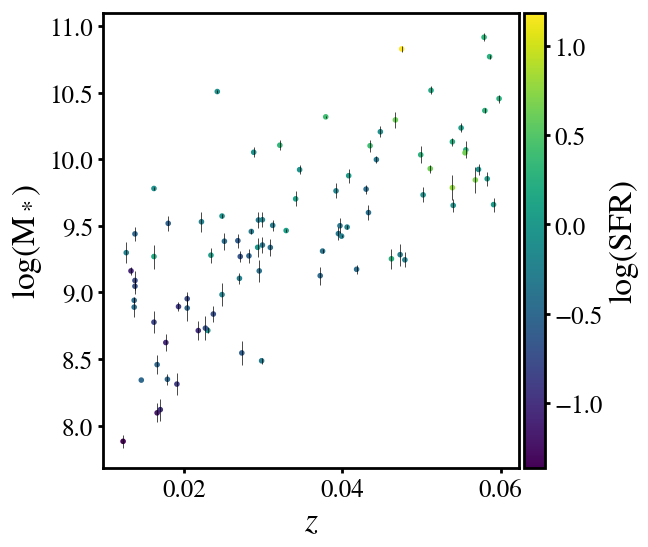
\includegraphics[width=5in]{Figures/mass_z_sfr.png}
\caption[Stellar mass, redshift, and Star-formation rate for a subset of our ``clumpy'' galaxies as measured by the GSWLC.]{Stellar mass, redshift, and star-formation rate (SFR) for a subset of 89 ``clumpy'' galaxies as measured by the GSWLC \citep{Salim2016}.}
\label{fig: clumpy gswlc properties}
\end{figure}

%The physical scale at z= 0.06 is 1"=1.1kpc. SDSS pixel scale is 0.396"/pixel. --> 0.43 kpc/pixel -->  ~2.3 pixels = 1kpc.  We visually inspect these spectra and verify that the fiber was positioned over a star-forming region in the majority of cases rather than the galactic bulge or other structure. 



\section{Are these star-forming regions analogs of high-redshift clumps?}
Many studies have been conducted (cite cite cite) comparing local HII regions to high-redshift star-forming clumps and the debate between whether these regions arise due to the same physical processes is still under debate. In this section we use the GSWLC and spectral features as measured by SDSS to explore various properties of the clumps in our sample. 


\subsection{Clump galactic radial distance} \label{subsec:radii}

Most SDSS fibers are either centered on a bright star-forming region or on/near the galactic center. We thus compute the galactocentric distance of each fiber from the galaxy center and normalized by the galaxy's half light radius (\texttt{FLUX\_RADIUS}) as determined by SExtractor. The resulting distribution is shown in the third panel of Figure \ref{fig: clump properties}. That the distribution is obviously skewed towards the small galactocentric values is likely due to the several spectra that are not covering a clump but instead probe the central region.  

 The \ha~equivalent width is a rough stand-in for specific SFR since it is the ratio of a strong star formation indicator (\ha~line flux) and a reasonable proxy for stellar mass, i.e., the stellar continuum at \ha \citep{MarmolQueralto2016}. However, we find no relation between EW(\ha) and clump radial distance. More telling would be a trend between clump radial distance and stellar age as this diagnostic will potentially distinguish between \textit{in situ} and external clump origin theories. The high quality of the SDSS spectra will allow for detailed stellar age estimates in a future analysis.  

\subsection{Clump luminosity}
We use the \ha~flux as measured by a Gaussian fit to the \ha~emission line to compute the star-formation rate using the well known calibration \citep[e.g.,][and references therein]{Calzetti2013}

\begin{equation}
\mathrm{SFR} (\mathrm{M}_{\odot} \mathrm{yr}^{-1}) = 5.5 \times 10^{-42}L(\mathrm{H}_{\alpha}) (\mathrm{ergs\ s}^{-1})
\end{equation}
 We can then compare SFRs between those derived from the \ha~emission and the global SED SFR. For each galaxy in the sample, we sum the SFR$_{\mathrm{H}_{\alpha}}$ from each spectrum and compare that to SFR$_{\mathrm{SED}}$, for those 89 galaxies that were matched to the GSWLC. Of those, we find the median ratio of the two star-formation measures is $\sim$10\%, with a majority of galaxies having only one spectrum which we interpret as one clump. This rough estimate is not dissimilar to giant star-forming regions found at high redshift where it is typical for individual clumps to contribute 10\% or more to the total star formation of the galaxy \citep{Genzel2011, Guo2012, Wisnioski2012}

\subsection{Velocity dispersion and clump diameters}

In the first panel of Figure \ref{fig: clump properties} we show the distribution of the \ha~velocity dispersion as measured by the SDSS spectroscopic pipeline, where the instrument resolution is subtracted in quadrature. The median for our sample is $\sigma_{\mathrm{H}_{\alpha}}\sim40$km/s and while this is slightly smaller than giant star-forming regions observed at $z\sim$2 (Sanchez et al., 2013; Elmegreen and Elmegreen, 2010), it is also significantly larger than typical HII regions observed in local galaxies (cite cite cite).

%A relationship between clump luminosity and velocity dispersion has been observed and it has been suggested that star formation drives the large observed line widths. In particular, Lehnert postulate that the velocity dispersion is due to mechanical energy released by star formation and that $\sigma$ is proportional to the star formation surface density. Another possibility is that the KS relation holds for star-forming regions


\begin{figure}
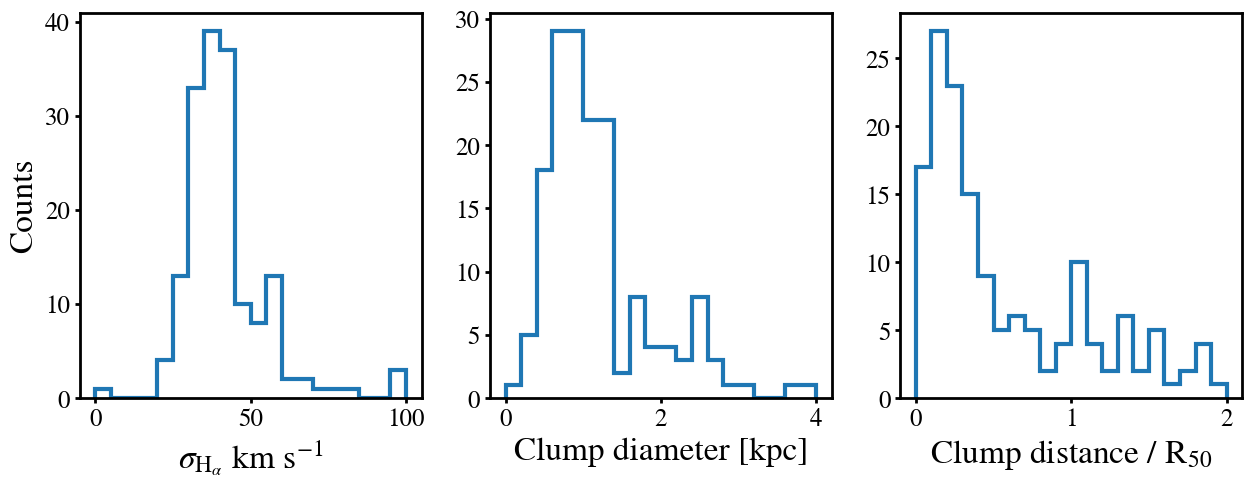
\includegraphics[width=\textwidth]{Figures/clump_properties.png}
\caption[Properties of ``clumps'': velocity dispersion, clump diameter, and clump galactic radial distance.]{Clump properties. }
\label{fig: clump properties}
\end{figure}


%\subsection{Clump diameters}
%If clumps form through disk instabilities as is traditionally thought, the relation between clump velocity dispersion and physical size can be theoretically derived as detailed in \citep[e.g.,][]{Wisnioski2012}, which we briefly review here. 

\cite{Wisnioski2012} develop empirical relations between clump size, luminosity, and velocity dispersion for a sample of local HII regions along with a sample of high redshift clumps. They demonstrate that these relations hold over three orders of magnitude in clump diameter and five orders of magnitude in \ha~luminosity for thousands of local HII regions and high-redshift clumps taken from 11 different studies. Specifically, we invert the following relation to estimate the clump diameter from the SDSS measurement of the \ha~velocity dispersion

\begin{equation}\label{eqn: clump diameter}
\log(\sigma) = (0.42 \pm 0.03) \times \log(d) + (0.33 \pm 0.09)
\end{equation}

The resulting clump diameter distribution is shown in the middle panel of Figure \ref{fig: clump properties}. The median diameter is $\sim$1 kpc which is larger than the average local HII region but slightly smaller than high redshift clumps.  Keep in mind that some of these ``clumps'' could actually be the central bulge region of some of these systems as we do not specifically separate the two so as to bias against the possibility of older (and hence redder, less star formation) clumps at smaller galactic radius. The central regions will typically have much lower rates of star formation as measured by \ha~and subsequently, smaller velocity dispersion, and thus they will have significantly smaller sizes according to this relation. In a more detailed analysis, clump sizes should be confirmed independently through a ``core'' analysis whereby clump sizes are measured by fitting a Gaussian to the 1D radial surface brightness profile of each star-forming region.  
%% If you wish to include an acknowledgments section in your paper,
%% separate it off from the body of the text using the \acknowledgments
%% command.



In future analyses, the quality of the SDSS spectra will allow for the derivation of accurate stellar ages from fitting of the continuum, as well as gas metallicity (e.g., Henry et al., 2015). With these measurements we can begin to study statistical properties that correlate with clump galactocentric distance. 

\section{Summary}


Though preliminary, this analysis demonstrates that star-forming regions in this galaxy sample are likely more similar to high-redshift clumps than to typical local HII regions. This motivates not only a more in depth analysis of this sample but also justifies the search for similar galaxies in the local universe. These clumpy galaxies were found as a consequence of SDSS Stripe 82 galaxies being included in the GZH project. We next detail a new project that will potentially find an order of magnitude more galaxies similar to the sample presented here.


%=========================================================================
%	CLUMP SCOUT
%=========================================================================
\section{Clump Scout}
The above analysis was performed on a subsample of galaxies determined as ``clumpy'' from the SDSS Stripe 82 sample included in the GZH project. The area covered by Stripe 82 was only a fraction of the full SDSS sky coverage. In this section we describe the \textit{Clump Scout} project, a citizen-science initiative to discover more ``clumpy'' galaxies in the remaining SDSS footprint. We thus consider the remaining non-Stripe 82 SDSS galaxies that were originally part of the GZ2 project. We first exclude any galaxies with $z>0.06$ in order to satisfy the resolution requirements discussed above. We also make a cut such that \fsmooth~$\le0.8$ in order to exclude those galaxies which are obviously elliptical and thus would likely not have travelled down the clumpy track of the GZH decision tree. These criteria yield a sample of $\sim63$K galaxies as shown in Figure \ref{fig: clump scout sample} where we depict galaxy number density contours in the $z$-\fsmooth plane. The red dashed lines denotes the \textit{Clump Scout} sample region. Based on the statistics of the clumpy galaxies found in the sky area of Stripe 82, we expect to find approximately 1000 such systems in the non-Stripe 82 SDSS sky coverage.

The goal of the project is to collect additional volunteer morphology information on par with that collected for the Stripe 82 sample in GZH. We will display jpeg images to volunteers via the Zooniverse Project Builder web platform which also hosts the Galaxy Zoo project.  However,  because we have such a large galaxy sample to go through, we will ask volunteers a slightly modified version of the top level question of the clumpy branch of the GZH decision tree in order to increase the speed of classification. Specifically, we ask one question, "Does the galaxy have a mostly clumpy appearance? If so, use the Clump Clicker tool to click the clumps you see." This takes advantage of the Zooniverse Point Tool which markes the location on the image with each click a volunteer makes. This will provide an affirmation of a clumpy galaxy, a preliminary clump count, and coarse clump localization information. We have already created a pilot version of this project which consisted of 1000 galaxy images in two different ``zoom'' levels and received favorable reviews from volunteers who participated. 

\begin{figure}
\centering
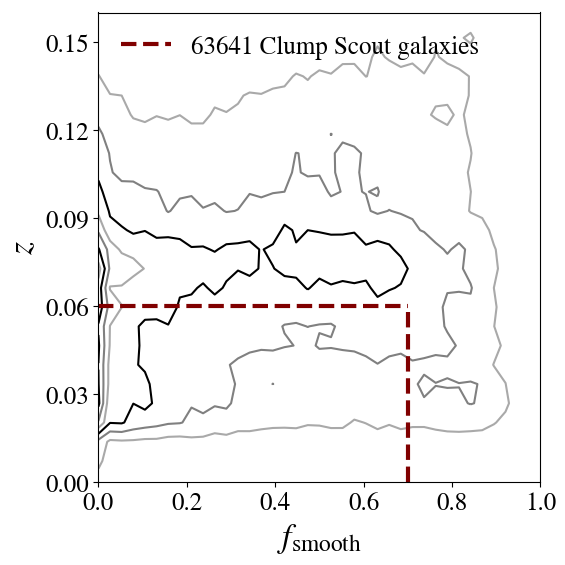
\includegraphics[width=5in]{Figures/clump_scout_sample_in_z-fsmooth.png}
\caption[\textit{Clump Scout} sample selection criteria from non-Stripe 82 GZ2 galaxy sample.]{\textit{Clump Scout} sample selection criteria from non-Stripe 82 GZ2 galaxy sample.}
\label{fig: clump scout sample}
\end{figure}



\subsection{Redshift evolution of \fclump}
With so many more clumpy galaxies at low redshift, we will be able to constrain clump origin formation theories. Specifically, we will investigate the evolution of the fraction of clumpy galaxies as a function of cosmic time, \fclump~(not to be confused with the GZH clumpy vote fraction). 

\cite{Guo2015} recently showed that the fraction of star-forming galaxies that have at least one off-center clump (\fclump) can be used to place constraints on theoretical models. By focusing on the redshift range between $0.5 <z<3$, they find that \fclump~changes with the stellar mass of the galaxies. Low-mass (M$<10$ 10 M) galaxies keep an almost constant fclumpy of $\sim$60\% from $z\sim3$ to $z\sim0.5$, while massive galaxies drop their \fclump~from 55\% at $z\sim3$ to 15\%, at $z\sim0.5$, as shown in Figure XXX \citep[adapted from][]{Guo2015}. \cite{Guo2015} argue that these observations support a model in which the clumpy star-formation results from multiple processes. In massive galaxies, the evolutionary trends are consistent with violent disk instability, however the apparent lack of \fclump~evolution in low mass galaxies is more consistent with a minor merger original. However, this conclusion, is based primarily on the lowest redshift bin probed by the \cite{Guo2015} data. In fact, when these data are combined with \fclump~measured from a variety of different surveys at $z<1$, the result is not so convincing anymore. The variation in the low-z measurements, however, is clearly large mostly as a consequence of non-uniform selection criteria and uncontrolled-for biases. \textit{Clump Scout} promises to provide the largest sample to date selected in a uniform fashion and with biases properly accounted for, especially in the low-mass regime where measurements of \fclump~can provide the strongest model constraints.

%In order to secure reliable measurements for \fclump~in the local universe, we must estimate the completeness of recovering low redshift clumpy galaxies from the SDSS sample. Ideally, we  To that end we need to conjure up some simulated clumpy galaxies that span the galactic mass and clump mass range appropriate for XXX reasons. 


\section{Summary and conclusions}
In this work, we have isolated a sample of galaxies with morphologies which resemble those of star-forming clumpy galaxies of the high-redshift universe. We identify these galaxies in the local universe through the Galaxy Zoo: Hubble project which included imaging from Stripe 82 of the SDSS. We isolate 105 galaxies that have a traditional clumpy morphology and acquire SDSS imaging and spectroscopic data for these galaxies, including spectra for over 150 clumps. We obtain stellar mass and star-formation rates for these galaxies through the GSWLC catalog. Through a preliminary analysis of the SDSS spectra we determine the clumps in these galaxies are in many ways consistent with high redshift clumps. However a more detailed analysis is necessary. 

Additionally, we describe the \textit{Clump Scout} project designed to search for additional clumpy galaxies in the local universe by presenting color-composite SDSS non-Stripe 82 imaging to the general public. We have made preliminary tests of this project with highly favorable reviews from volunteers and we expect to find an additional 1000 clumpy galaxies. This will provide a large statistical sample of local clumpy galaxies which will constrain the fraction of clumpy galaxies at low redshift allowing us to distinguish between various clump original theories. Additionally, because these are all SDSS objects, there will undoubtedly be spectra for thousands of clumps allowing for large statistical studies of star formation in the nearby universe. 